% \clearpage
\section{More experiment results}
\label{section:more_experiment_results}

\subsection{Comparison on convergence speed and generalization}

We include the missing figures of Section~\ref{section:experiments}. Results on other datasets and the discussion on the experiment results could be found next to Figure~\ref{fig:train_extra_wiki_lastfm_gdelt_ne}.

\begin{figure}[h]
\centering
\begin{subfigure}{0.32\textwidth}
    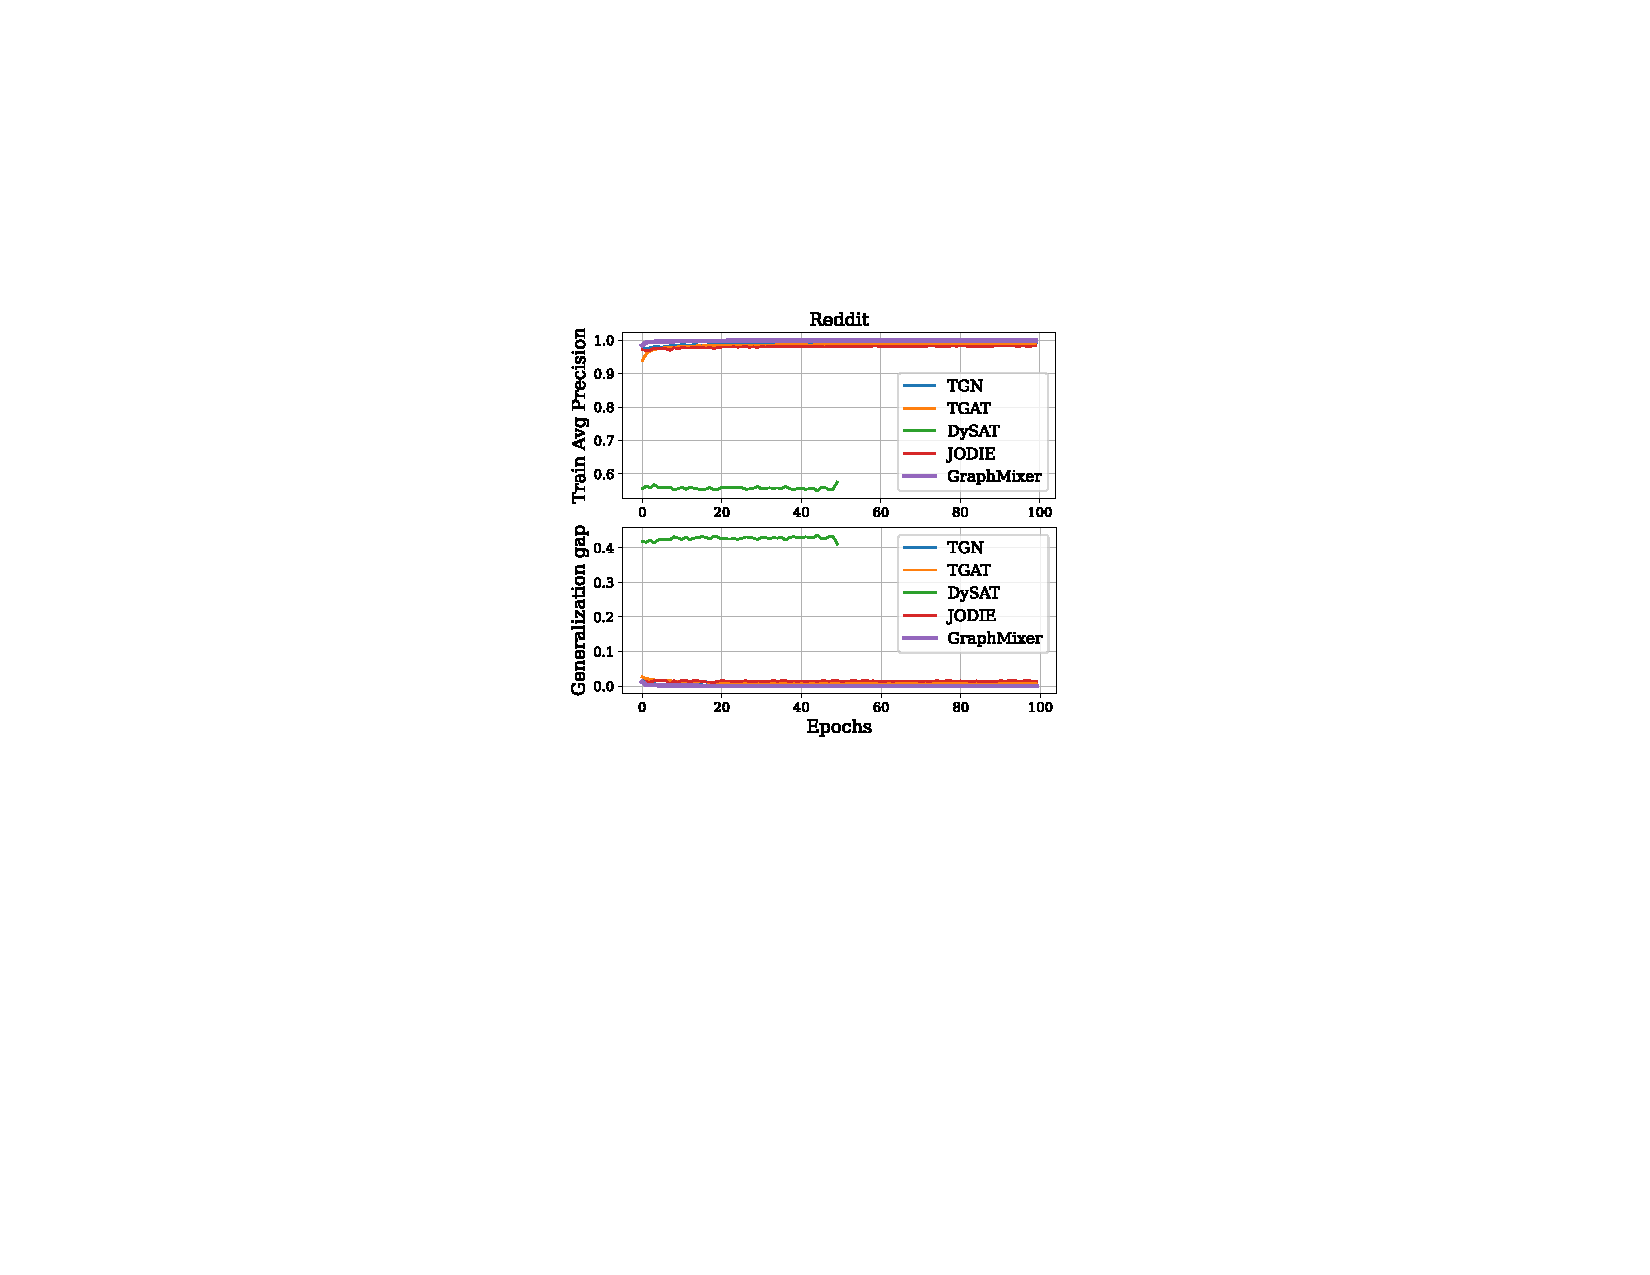
\includegraphics[width=\textwidth,height=3.5cm]{figures/train_extra/reddit_train_extra.pdf}
    \vspace{-6mm}
    % \caption{Evaluation average precision}
    % \label{fig:first}
\end{subfigure}
\hspace{0cm}
\begin{subfigure}{0.32\textwidth}
    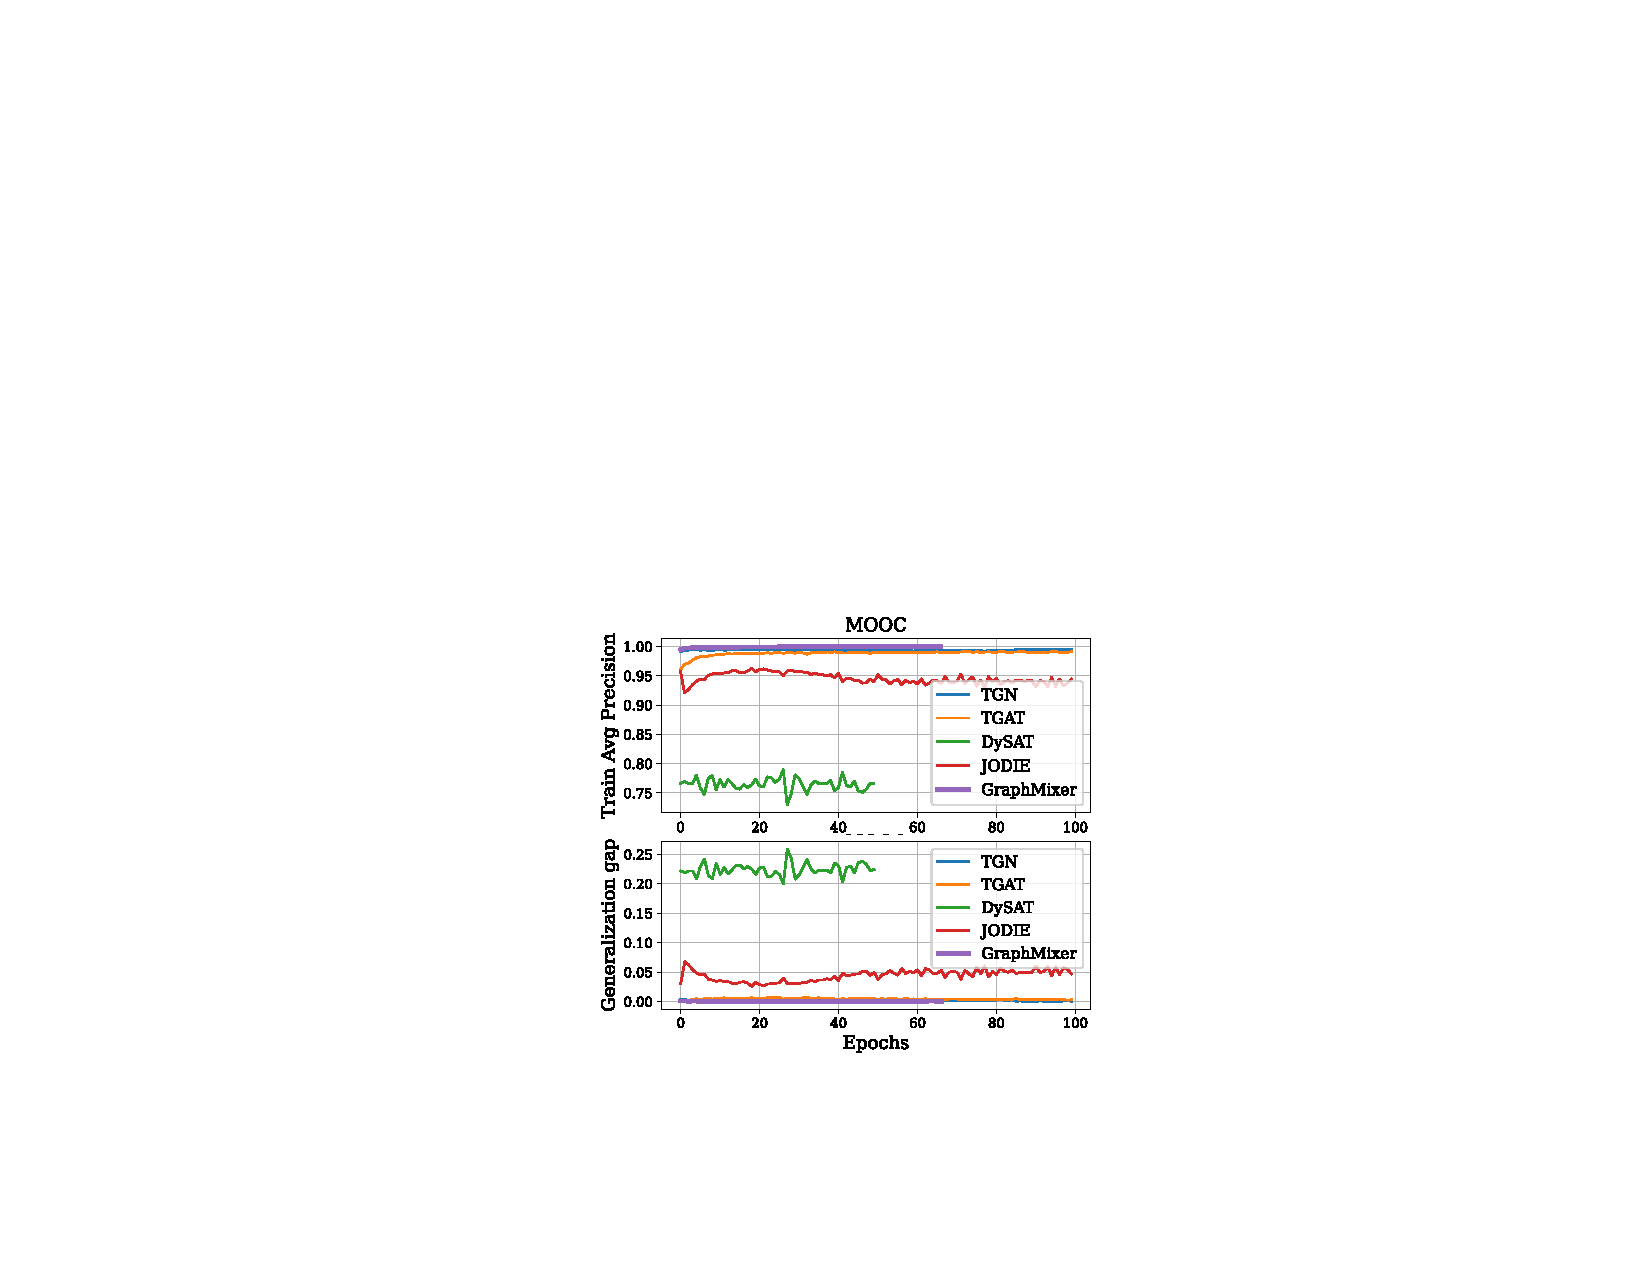
\includegraphics[width=\textwidth,height=3.5cm]{figures/train_extra/mooc_train_extra.pdf}
    \vspace{-6mm}
    % \caption{Train average precision}
    % \label{fig:second}
\end{subfigure}
\hspace{0cm}
\begin{subfigure}{0.32\textwidth}
    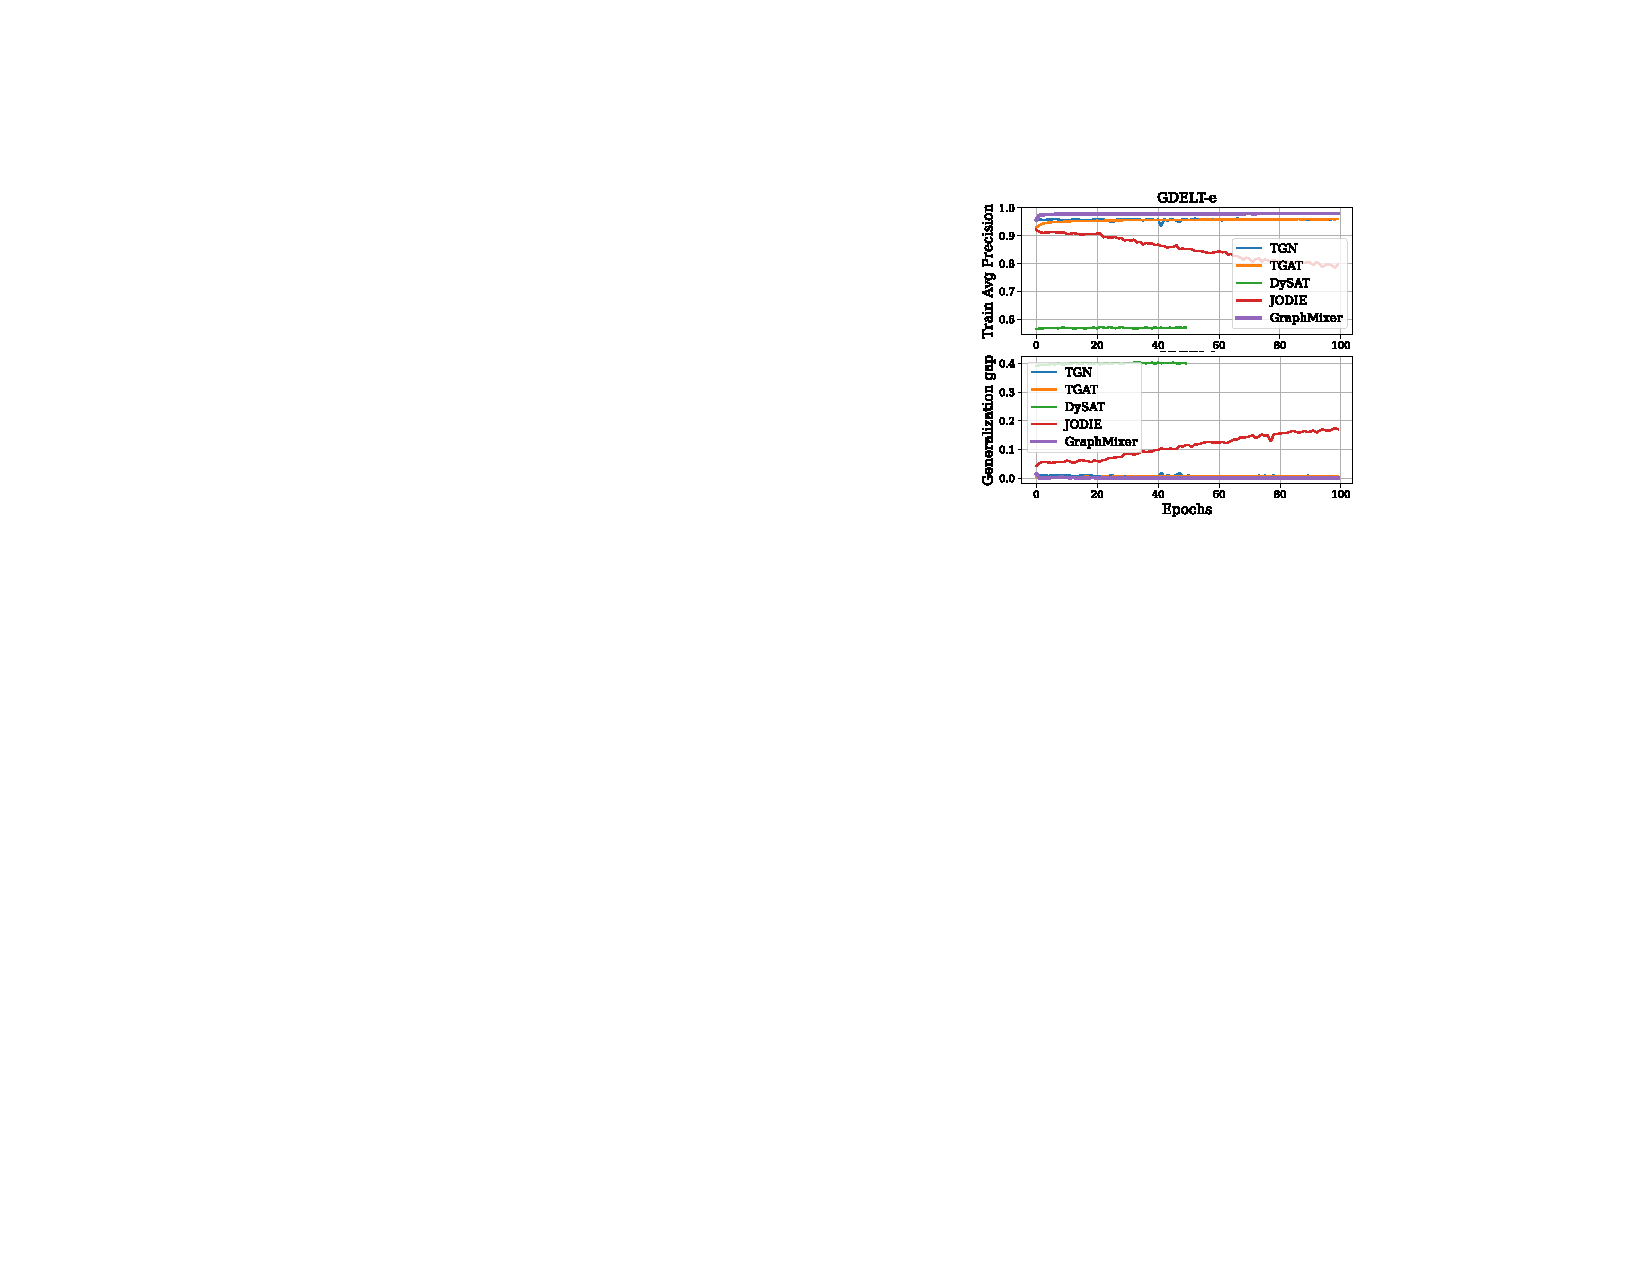
\includegraphics[width=\textwidth,height=3.5cm]{figures/train_extra/gdelt_e_train_extra.pdf}
    \vspace{-6mm}
    % \caption{Generalization gap}
\end{subfigure}
\vspace{-2mm}
\caption{Comparison of the link prediction training average precision and generalization gap for the first $100$ training epochs. Results on other datasets can be found in Figure~\ref{fig:train_extra_wiki_lastfm_gdelt_ne}.}
\label{fig:train_extra_reddit_mooc_gdelt_e}
\end{figure}

% \clearpage
% \subsection{Missing results for Section~\ref{section:data_alignment}}

% \begin{table}[h]
% \caption{Comparison on the average precision score of \our with different input data. The highlighted rows are using default setting as we used.
% } % and  Hits$@$K 
% \label{table:average_precision_input_data_quality}
% \vspace{-3mm}
% \centering
% \scalebox{0.85}{
% \begin{tabular}{ l rr  ll ll  }
% \hline\hline
%   & & & Reddit & Wiki & MOOC & LastFM \\ \hline\hline
% \multirow{4}{*}{\begin{tabular}[c]{@{}l@{}}Time\\ information\end{tabular}}       & \multicolumn{2}{r}{Relative timestamp $(t_i-t_0)$} & $99.79$ & $99.80$ &  $99.91$ & $95.32$           \\
%                                                                               & \multicolumn{2}{r}{Relative time-feats $\cos((t_i-t_0)\boldsymbol{\omega})$} & \cellcolor[HTML]{FEDEDC}$99.93$ & \cellcolor[HTML]{FEDEDC}$99.85$ & \cellcolor[HTML]{FEDEDC}$99.91$ &  \cellcolor[HTML]{FEDEDC}$96.31$  \\
%                                                                               & \multicolumn{2}{r}{Absolute timestamp $t_i$} &        &      &      &                  \\
%                                                                               & \multicolumn{2}{r}{Absolute time-feats $\cos(t_i\boldsymbol{\omega})$} &        &      &      &                 \\ \hline
% \multirow{4}{*}{\begin{tabular}[c]{@{}l@{}} Neighbor \\ selection \end{tabular}} & 2-hop & Most recent neighbors   &   99.39     &   98.05   &   99.11   &  89.36            \\
%                                                                               & 1-hop & Most recent neighbors& \cellcolor[HTML]{FEDEDC}$99.93$ & \cellcolor[HTML]{FEDEDC}$99.85$ & \cellcolor[HTML]{FEDEDC}$99.91$ &  \cellcolor[HTML]{FEDEDC}$96.31$ \\
%                                                                               & 2-hop & Uniform sample  neighbors  & $97.66$ &  $92.57$ &  $98.87$    &     $65.72$    \\
%                                                                               & 1-hop & Uniform sample neighbors   &  $98.19$ & 94.74     &  $98.40$     &     $60.02$            \\\hline
% \hline
% \end{tabular}}
% \end{table}


\subsection{Transductive learning with Recall@K and MRR as evaluation metric}
Recall@K and MRR (mean reciprocal rank) are popular evaluation metrics used in the real-world recommendation system. The larger the numbers, the better the model performance.
Our Recall@K and MRR is implemented based on the Open Graph Benchmark's link prediction evaluation metrics' implementation\footnote{\url{https://github.com/snap-stanford/ogb/blob/master/ogb/linkproppred/evaluate.py}}. More specifically, we first sample $100$ negative destination nodes for the source node of each temporal link node pair, then our goal is to rank the positive temporal link node pairs higher than 100 negative destination nodes.
In the following, we compare the Recall@5 and MRR score of \our with the selected four most representative baselines.
Please notice that since these methods are implemented under the same framework, the model performance is evaluated by using the same model used in Table~\ref{table:average_precision}, the comparison is guaranteed to be fair.

\begin{table}[h]
\caption{Comparison on the Recall@K and MRR.}
\label{table:recall_mrr}
\vspace{-3mm}
\centering
\scalebox{0.8}{
\begin{tabular}{ l | cc | cc | cc | cc | cc}
\hline\hline
       & \multicolumn{2}{c|}{Reddit} & \multicolumn{2}{c|}{Wiki} & \multicolumn{2}{c|}{MOOC} & \multicolumn{2}{c|}{LastFM} & \multicolumn{2}{c}{GDELT}   \\
    %   & Node / links & 11K/7M & 9K/6M & 7K/4M & 2K/1.3M & 9K/2M & 9K/2M & 9K/2M \\
    %   & Links per node & 61.2 & 17.1 & 57.6 & 653.1 & 216.6 & 216.6 & 216.6 \\ 
      & R@5 & MRR & R@5 & MRR & R@5 & MRR & R@5 & MRR & R@5 & MRR \\ \hline\hline
JODIE & $0.9181$ & $0.6271$ & $0.9098$ & $0.7752$ & $0.9818$ & $0.7551$ & $0.2034$ & $0.1206$ & $0.8554$ & $0.6048$  \\ 
DySAT & $0.9189$ & $0.7774$ & $0.8889$ & $0.7561$ & $0.9989$ & $0.7906$ & $0.4159$ & $0.3322$ & $0.8302$ & $0.4236$ \\ 
TGAT  & $0.9774$ & $0.8709$ & $0.8508$ & $0.6132$ & $0.9736$ & $0.7425$ & $0.1040$ & $0.0769$ & $0.3513$ & $0.2366$ \\  
TGN   & $0.9787$ & $0.9093$ & $0.8878$ & $0.8016$ & $0.9904$ & $0.9904$ & $0.1649$ & $0.1153$ & $0.9297$ & $0.7295$ \\ 
\our  & $\mathbf{1.0}$ & $\mathbf{0.9965}$ & $\mathbf{0.9972}$ & $\mathbf{0.9876}$ & $\mathbf{0.9999}$ & $\mathbf{0.9910}$ & $\mathbf{0.9998}$ & $\mathbf{0.9649}$ &  $\mathbf{0.9930}$ & $\mathbf{0.8934}$ \\  
\hline\hline
\end{tabular}}
\end{table}

We have the following observations on Table~\ref{table:average_precision}:
\begin{itemize} [noitemsep,topsep=0pt,leftmargin=2mm ]
    \item According to the results in Table~\ref{table:recall_mrr}, \our could achieve outstanding performance across all datasets. Especially on the LastFM and GDELT datasets (denser graphs than other datasets). This might implies \our is more suitable for denser graphs than other baseline methods.
    \item The results of some baseline methods behave less better with Recall@K and MRR evaluation metrics. For example, TGN on LastFM dataset, TGAT on LastFM and GDELT, etc. The above results also imply the limitation of only considering average precision and AUC score for temporal link evaluation.
\end{itemize}





\clearpage
\subsection{Comparison on wall-clock time} \label{section:wall_clock_time}

In the following, we compare the wall-clock time it takes for \our and baselines to finish a single epoch of training. 

\begin{table}[h]
\caption{Comparison on the wall-clock computation time for single-epoch of training. 
% \textcolor{red}{For \oure, we report both the computation time (outside parenthesis) and data mini-batch preparation time (inside parenthesis) for the completeness.
}
\label{table:compute_time}
\vspace{-4mm}
\centering
\centering\setlength{\tabcolsep}{6mm}
\scalebox{0.85}{
\begin{tabular}{ l cccc c}
\hline\hline
      & Reddit & Wiki & MOOC & LastFM & GDELT  \\
    %   & Node / links & 11K/7M & 9K/6M & 7K/4M & 2K/1.3M & 9K/2M & 9K/2M & 9K/2M \\
    %   & Links per node & 61.2 & 17.1 & 57.6 & 653.1 & 216.6 & 216.6 & 216.6 \\ 
      \hline\hline
JODIE & $5$ sec & $2$ sec & $4$ sec & $11$ sec & $16$ sec \\ 
DySAT & $33$ sec & $6$ sec & $16$ sec & $41$ sec & $83$ sec \\ 
TGAT  & $15$ sec & $4$ sec & $8$ sec & $28$ sec & $41$ sec \\  
TGN   & $8$ sec & $2$ sec & $5$ sec & $15$ sec & $32$ sec \\  \hline
CAWs-mean & $1,893$ sec & $277$ sec & $641$ sec & $1,797$ sec & $4,544$ sec \\  
CAWs-attn  & $1,930$ sec & $282$ sec & $653$ sec & $1,832$ sec & $4,634$ sec \\  
TGSRec & $538$ sec & $157$ sec & $656$ sec & $1,810$ sec & $3,707$ sec \\  
APAN & $13$ sec & $4$ sec & $9$ sec & $28$ sec & $25$ sec \\ \hline 
% \our & $53$ sec & $12$ sec & $27$ sec & $69$ sec & $103$ sec \\ 
\our & $12$ sec & $3$ sec & $7$ sec & $21$ sec & $32$ sec \\ 
% \textcolor{red}{\our} & \textcolor{red}{$12~(41)$ sec} & \textcolor{red}{$3~(9)$ sec} & \textcolor{red}{$7~(20)$ sec} & \textcolor{red}{$21~(48)$ sec} & \textcolor{red}{$32~(71)$ sec} \\ 
\hline\hline
\end{tabular}}
\vspace{-3mm}
\end{table}

When comparing the computation time of \our with CAWs, TGSRec, and DDGCL, we found that \our takes significantly lesser time than these baselines, which indicates the effectiveness of \oure.
When comparing the computation time of \our with JODIE, DySAT, TGAT, APAN, and TGN, we found that \our  is very close to or even slightly faster than some baseline methods. Our computation time is slightly slower than other baseline methods (e.g., JODIE and TGN) mainly because these baselines are using well-optimized computation functions from DGL~\cite{wang2019dgl}, while \our is just using a composition of basic PyTorch functions.
In fact, according to the Table~\ref{table:number_of_params}, \our has a similar/smaller amount of parameters with these baselines.

\begin{table}[h]
\centering
\caption{Comparison on the number of model parameters. }\label{table:number_of_params}
\vspace{-3mm}
\scalebox{0.85}{
\begin{tabular}{ l | c c c | c c c c}
\hline\hline
                     & \our & \oure-T & \oure-S & Jodie & DySAT & TGAT & TGN \\ \hline\hline
\# Parameters ($\times 10^5$) &  2.25   &  1.42  &  2.07 & 1.21 & 9.38 & 3.80 & 3.54 \\ \hline\hline
\end{tabular}}
\vspace{-2mm}
\end{table}


% Besides, from the last row of Table~\ref{table:compute_time}, we know that our computation time (outside parenthesis) is much smaller than the data mini-batch preparation time (inside parenthesis). 
% Due to limitation on computational resources, we process the data for each epoch of training.
Besides, our current implementation also need to preprocess the input data for each epoch of training, e.g., sorting nodes in subgraph according to temporal order and removing duplicated edges.
For example, the data preparation at each epoch takes 41 sec on Reddit, 9 sec on Wiki, 20 sec on MOOC, 48 sec on LastFM, and 71 sec on GDELT. 
However, by caching the pre-processed data in the memory, we only need to pre-process the input data at the first epoch of the training process because our neighbor selection is deterministic and the input data does not change at each epoch.
% However, due to limitation on computational resources, we cannot cache all the input data in memory for large dataset, and choose to preprocess the input data for each epoch of training.





% \clearpage
\subsection{Transductive learning with AUC as evaluation metric} \label{section:transductive_AUC_score}
AUC (Under the ROC Curve) is one of the most widely accepted evaluation metric for link prediction, which has been used in many existing works~\cite{xu2020inductive,tgn_icml_grl2020}.
In the following, we compare the AUC score of \our with baselines.
We have the following observations: 
\circled{1} \our outperforms all baselines on all datasets. In particular, \our attains more than $1\%$ gain over all baselines on the \textit{LastFM}, \textit{GDELT-ne}, and \textit{GDELT-e} datasets, attains around $2\%$ gain over non-RNN methods \textit{DySAT} and \textit{TGAT} on the \textit{Wiki} dataset, and attains around $11\%$ gain over non-RNN methods \textit{DySAT} and \textit{TGAT} on the \textit{GDELT-ne} dataset. The experiment results provide sufficient support on our argument that neither RNN nor SAM is necessary for temporal graph link prediction.
\circled{2} According to the performance of \oure-L on datasets only have link timestamp information (\textit{MOOC}, \textit{LastFM}, and \textit{GDELT-ne}), we know that our time-encoding function could successfully pre-process each timestamp into a meaningful vector. 
\circled{3} By comparing the performance \oure-N and \our on \textit{Wiki}, \textit{MOOC}, and \textit{LastFM} datasets, we know that node-info encoder alone is not enough to achieve a good performance. However, it provides useful information that could benefit the link-info encoder.
\circled{4} By comparing the performance of \oure-N on \textit{GDELT} and \textit{GDELT-ne}, we observe that using one-hot encoding outperforms using node features. This also shows the importance of node identity information because one-hot encoding only captures such information. 

\begin{table}[h]
\caption{Comparison on the AUC score for link prediction. \our uses one-hot node encoding for datasets without node features (marked by $\natural$). For each dataset we indicate whether we have the corresponding feature (``L'' link features, ``N'' node features, and ``T'' link timestamps).
% and the average number of temporal links per node in the dataset.
}  % and  Hits$@$K , baselines either uses link features and time features (marked by $$) or uses random features  (marked by $$) as node features  
\label{table:transductive_AUC_score}
\vspace{-4mm}
\centering
\centering\setlength{\tabcolsep}{1mm}
\scalebox{0.8}{
\begin{tabular}{ l cccc ccc}
\hline\hline
       & Reddit & Wiki & MOOC & LastFM & GDELT & GDELT-ne & GDELT-e \\
       & L, T & L, T & T & T & L, N, T & T & N, T \\
    %   & Node / links & 11K/7M & 9K/6M & 7K/4M & 2K/1.3M & 9K/2M & 9K/2M & 9K/2M \\
    %   & Links per node & 61.2 & 17.1 & 57.6 & 653.1 & 216.6 & 216.6 & 216.6 \\ 
      \hline\hline
JODIE & $99.30 \pm 0.01$ & $98.81 \pm 0.01$ & $99.16 \pm 0.01$ & $67.51 \pm 1.99$ & $98.55 \pm 0.01$ & $97.13 \pm 0.02$ & $96.96 \pm 0.02$ \\ 
DySAT & $98.52 \pm 0.01$ & $96.71 \pm 0.02$ & $98.82 \pm 0.01$ & $76.40 \pm 0.81$ & $98.52 \pm 0.01$ & $82.47 \pm 0.04$ & $97.25 \pm 0.02$\\ 
TGAT  &  $99.66 \pm 0.01$ & $97.75 \pm 0.02$ & $98.43 \pm 0.01$ & $54.77 \pm 1.02$ & $98.25 \pm 0.01$ & $84.30 \pm 0.03$ & $96.96 \pm 0.02$ \\ 
TGN   &  $99.80 \pm 0.01$ & $99.55 \pm 0.01$ & $99.62 \pm 0.01$ & $82.23 \pm 0.50$ & $98.15 \pm 0.01$ & $97.13 \pm 0.02$ & $96.04 \pm 0.02$ \\ \hline
CAWs-mean& $98.18 \pm 0.01$ & $97.25 \pm0.03$ & $63.88\pm0.92$ & $72.92 \pm 0.33$ & $95.19 \pm 0.09$ & $71.82 \pm 0.08$ & $91.40 \pm 0.19$\\
CAWs-attn& $98.30 \pm 0.01$ & $97.89 \pm0.02$ & $63.95\pm0.81$ & $72.93 \pm 0.54$ & $95.13 \pm 0.11$ & $71.82 \pm 0.08$ & $91.64 \pm 0.24$ \\
TGSRec & $94.74 \pm 0.20$ & $91.32 \pm 0.19$ & $80.70 \pm 2.31$ & $76.66 \pm 1.54$ & $96.72 \pm 0.42$ & $96.72 \pm 0.42$ & $96.72 \pm 0.42$\\
APAN & $99.24 \pm 0.01$ & $97.25 \pm 0.01$ & $98.58 \pm 0.01$ & $62.73 \pm 0.64$ & $96.46 \pm 0.11$ & $98.39 \pm 0.17$ & $97.85 \pm 0.19$\\\hline 
\oure-L &  $99.84 \pm 0.01$ & $99.70 \pm 0.01$ & $99.87 \pm 0.01$ & $97.04 \pm 0.02$ & $\textbf{98.99} \pm 0.02$ & $96.54 \pm 0.02$ & $\textbf{98.99} \pm 0.02$ \\ 
\oure-N &  $99.53 \pm 0.01^\natural$ & $91.49 \pm 0.01^\natural$ & $98.66 \pm 0.02^\natural$ & $71.51 \pm 0.03^\natural$ & $94.44 \pm 0.02$ & $96.00 \pm 0.02^\natural$ & $98.81 \pm 0.02^\natural$ \\ 
\our &  $\mathbf{99.94} \pm 0.01^\natural$ & $\textbf{99.82} \pm 0.01^\natural$ & $\textbf{99.93} \pm 0.01^\natural$ &  $\textbf{97.38} \pm 0.02^\natural$ & $98.89 \pm 0.02$ & $\textbf{98.50} \pm 0.02^\natural$ & $98.48 \pm 0.02^\natural$ \\ 
% JODIE & (Fixed time-encoder)     & 9976 & 9900 & 9917 & 7989 & & 9696    \\ 
% TGAT & (Fixed time-encoder)     & 9948 & 9855 & 9933 & 7626 & & 9628    \\
% TGN & (Fixed time-encoder)     & 9983 & 9954 & 9962 & 8758 & & 9734    \\ 
\hline\hline
\end{tabular}}
\vspace{-4mm}
\end{table}


% \subsection{Inductive learning with AP and AUC as evaluation metric}

% \weilin{give an introduction on inductive learning setting + how we did this}

% \begin{table}[h]
% \caption{Comparison on the AP and AUC under inductive learning setting. \weilin{the table need to fill in}}
% \label{table:inductive_learning}
% \vspace{-3mm}
% \centering
% \scalebox{0.8}{
% \begin{tabular}{ l | cc | cc | cc | cc | cc}
% \hline\hline
%       & \multicolumn{2}{c|}{Reddit} & \multicolumn{2}{c|}{Wiki} & \multicolumn{2}{c|}{MOOC} & \multicolumn{2}{c|}{LastFM} & \multicolumn{2}{c}{GDELT}   \\
%     %   & Node / links & 11K/7M & 9K/6M & 7K/4M & 2K/1.3M & 9K/2M & 9K/2M & 9K/2M \\
%     %   & Links per node & 61.2 & 17.1 & 57.6 & 653.1 & 216.6 & 216.6 & 216.6 \\ 
%       & AP & AUC & AP & AUC & AP & AUC & AP & AUC & AP & AUC \\ \hline\hline
% JODIE & $0.0000$ & $0.0000$ & $0.0000$ & $0.0000$ & $0.0000$ & $0.0000$ & $0.0000$ & $0.0000$ & $0.0000$ & $0.0000$  \\ 
% DySAT & $0.0000$ & $0.0000$ & $0.0000$ & $0.0000$ & $0.0000$ & $0.0000$ & $0.0000$ & $0.0000$ & $0.0000$ & $0.0000$  \\ 
% TGAT  & $0.0000$ & $0.0000$ & $0.0000$ & $0.0000$ & $0.0000$ & $0.0000$ & $0.0000$ & $0.0000$ & $0.0000$ & $0.0000$  \\ 
% TGN   & $0.0000$ & $0.0000$ & $0.0000$ & $0.0000$ & $0.0000$ & $0.0000$ & $0.0000$ & $0.0000$ & $0.0000$ & $0.0000$  \\  
% \our  & $\mathbf{99.95}$ & $\mathbf{99.91}$ & $\mathbf{99.79}$ & $\mathbf{99.59}$ & $\mathbf{99.99}$ & $\mathbf{99.98}$ & $\mathbf{0.0000}$ & $\mathbf{0.0000}$ &  $\mathbf{0.0000}$ & $\mathbf{0.0000}$ \\  
% \hline\hline
% \end{tabular}}
% \end{table}

% \weilin{this part is not very necessary i think, if we still have time after i am done with transduction experiments, i might work on this part.
% }


% \clearpage

\subsection{Baselines with undirected temporal graph} \label{section:baseline_undirected}

\our utilizes undirected temporal graph to capture whether two nodes are frequently connected in the last few timestamps. In the following, we test whether using undirected temporal graph could improve the performance of baseline methods.
As we can see from Table~\ref{table:baseline_undirected}, using undirected temporal graph cannot improve the performance of baseline methods much because such information are already implicitly captured via their neural architecture design or sampling methods.

\begin{table}[h]
\caption{Comparison on baselines with undirected temporal graph (Average precision~|~AUC score).}
\label{table:baseline_undirected}
\vspace{-4mm}
\centering
\scalebox{0.85}{
\begin{tabular}{ l cccc }
\hline\hline
       & Reddit & Wiki & MOOC & LastFM \\
    %   & Node / links & 11K/7M & 9K/6M & 7K/4M & 2K/1.3M & 9K/2M & 9K/2M & 9K/2M \\
    %   & Links per node & 61.2 & 17.1 & 57.6 & 653.1 & 216.6 & 216.6 & 216.6 \\ 
      \hline\hline
JODIE & $99.24~|~99.40$ & $98.91~|~99.07$ & $99.18~|~99.53$ & $73.25~|~80.24$ \\ 
DySAT & $98.53~|~98.42$ & $96.61~|~96.88$ & $98.80~|~99.26$ & $76.23~|~73.90$  \\ 
TGAT  & $99.70~|~99.73$ & $97.35~|~97.68$ & $98.41~|~98.85$ & $54.58~|~57.03$  \\  
TGN   & $99.84~|~99.87$ & $99.59~|~99.61$ & $99.44~|~99.66$ & $91.96~|~93.20$  \\ 
\hline\hline
\end{tabular}}
\vspace{-4mm}
\end{table}

\section{Discussion about model performance on LastFM}

Our results show that \our could outperform baselines on LastFM dataset with a large margin, which is due to a composite effect of multiple factors. In the following, we summarize several potential factors that lead to our observation on the model performance.
\begin{itemize} [noitemsep,topsep=0pt,leftmargin=5mm ]
    \item \textbf{Larger average time-gap.} LastFM has a larger average time-gap $(t_{\max} - t_{\min})/|\mathcal{E}|$ than other datasets. As shown in the dataset statistic (Table~\ref{table:dataset_stat}), LastFM has an average time gap of 106, which is significantly larger than other datasets. For example, Reddit's average time gap is $4$, Wiki's average time gap is $17$, MOOC's average time gap is $3.6$, and GDELT's average time gap is $0.1$. Since baseline methods are relying on RNN and SAM to process the historical temporal information, they implicitly assumes the temporal information is ``smooth'' and with smaller average time gap. Therefore, baseline methods could potentially work better on the dataset with a smaller average time gap but are less ideal on LastFM. \our is not relying on RNN or SAM, therefore could be less affected by the aforementioned issue.
    \item \textbf{Larger average node degree.} LastFM has a larger average node degree $|\mathcal{E}|/|\mathcal{V}|$ than other datasets, which potentially prone to over-smoothing (aggregating features from many neighbors make output representation less distinguishable~\cite{li2018deeper}), over-squashing (aggregating much information into a limited memory might compress too much useful information~\cite{alon2020bottleneck}) and over-fitting~\cite{cong2021provable} effect. For example, according to the dataset statistic in Table~\ref{table:dataset_stat}, LastFM has an average node degree of $653$, which is larger than the Reddit's average node degree $61$, Wiki's average node degree $17$, MOOC's average node degree $57$, and GDELT's average node degree $216$. Existing methods either use the memory cell in RNN to store temporal information or use SAM to aggregate temporal information from multi-hops, which could be less ideal on a dense graph due to over-smoothing and over-squashing. However, \our is less relying on the aggregation schema, therefore its performance is better than the baseline methods. 
    % \item LastFM dataset consists of information on who listens-to-which song, where the 1-hop recent neighbors information might be more important than other dataset.
    % For example as shown in Table~\ref{table:average_precision_input_data_quality} and discussed in Section~\ref{section:data_alignment}, changing the neighbor selection scheme and change undirected graph to directed graph could also largely affect the model performance of \oure.
    \item \textbf{Larger maximum timestamp.} GraphMixer is using fixed time encoder but baselines are using trainable time-encoders. Since the largest timestamp $t_{\max}$ in LastFM is larger than other datasets, the trainable time-encoder is more affected by the unbounded gradient issue as discussed in Table~\ref{table:average_precision_baselines_fixed_time_encoder} and Section~\ref{section:time_encoder}. For example, the $t_{\max}$ in LastFM is 137 millon, while $t_{\max}$ in GDELT 0.2 millon, $t_{\max}$ in Reddit 2.6 millon, $t_{\max}$ in Wiki 2.6 millon, and $t_{\max}$ in MOOC 2.6 millon.
\end{itemize}
